\chapter{Schematic Converter in eSim}
\thispagestyle{empty}
\label{chap13}

\section{Schematic Converter in eSim}
\label{sec:schematic-converters}

eSim provides schematic converters to assist users in importing schematics from widely used proprietary EDA tools like \textbf{LTspice} and \textbf{PSpice} into eSim’s open-source environment. These converters reduce the friction involved in transitioning to open-source workflows and allow reuse of existing designs.

\subsection{Purpose}
Schematic converters enable users to convert schematics from commercial tools into a format compatible with eSim, which is based on KiCad and Ngspice. This supports:

\begin{itemize}
  \item Migration from proprietary to open-source tools
  \item Reuse of existing circuits and designs
  \item Seamless integration into the eSim project workspace
\end{itemize}

\subsection{Available Converters}

The converters are located in the eSim source directory at:

\begin{verbatim}
/src/converter
\end{verbatim}

\begin{itemize}
  \item \textbf{LTSpiceToKiCadConverter:}
  \begin{itemize}
    \item Converts \texttt{.asc} files from LTspice to KiCad compatible schematics used in eSim.
    \item Translates component symbols, wiring, and schematic layout.
    \item Located in:
    \begin{verbatim}
    /src/converter/LTSpiceToKiCadConverter/
    \end{verbatim}
    \item Separate codebases for:
    \begin{itemize}
      \item Windows: \texttt{src/Windows/}
      \item Ubuntu/Linux: \texttt{src/Ubuntu/}
    \end{itemize}
  \end{itemize}

  \item \textbf{PSpiceToKiCadConverter:}
  \begin{itemize}
    \item Converts \texttt{.sch} files from PSpice into eSim format.
    \item Maps PSpice components to equivalent KiCad symbols and extracts netlist connections.
    \item Located in:
    \begin{verbatim}
    /src/converter/PSpiceToKiCadConverter/
    \end{verbatim}
  \end{itemize}
\end{itemize}

\subsection{How It Works}
Each converter uses a Python-based parser to extract schematic information and create a new project folder containing KiCad-compatible files. The steps are:

\begin{enumerate}
  \item Parse the source schematic (\texttt{.asc} or \texttt{.sch}).
  \item Extract components, wires, labels, and attributes.
  \item Map components to eSim-compatible symbols.
  \item Generate the necessary schematic files.
  \item Copy the converted schematic into the user's eSim workspace.
\end{enumerate}

\subsection{Integration with eSim GUI}
The schematic conversion is fully integrated into the eSim graphical interface. Users can:
\begin{figure}
    \centering
    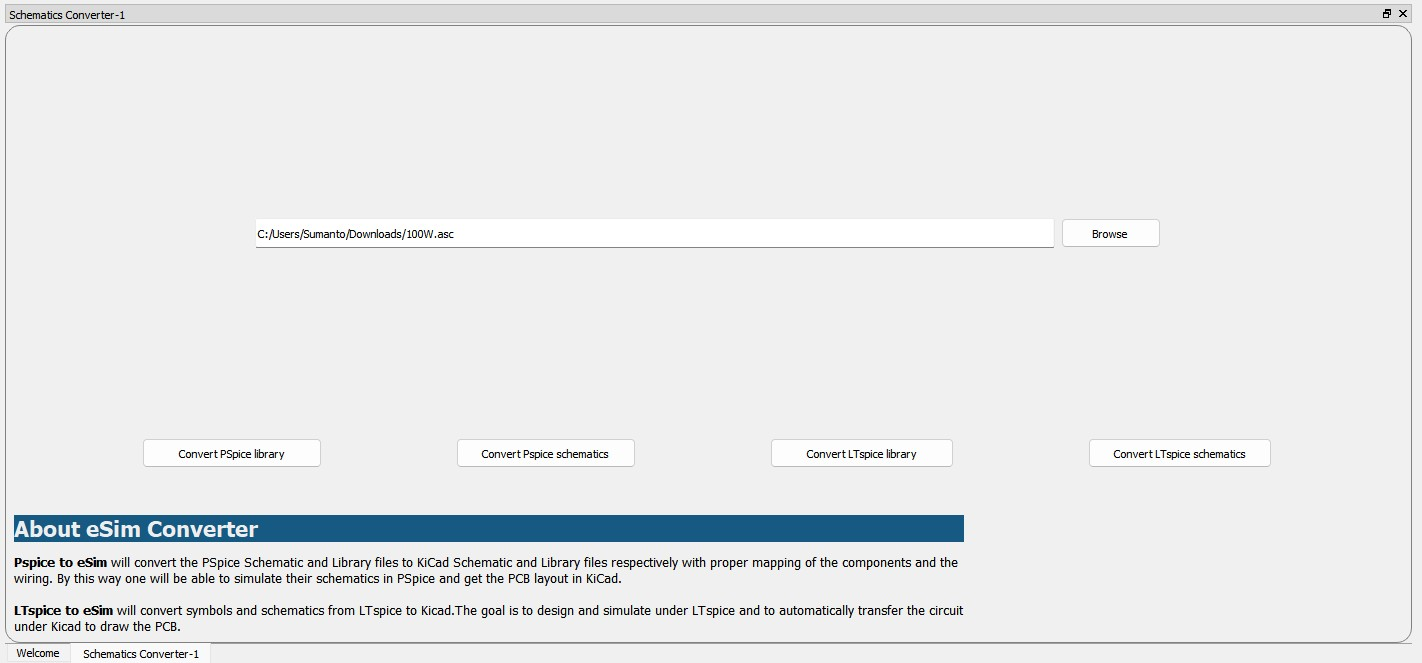
\includegraphics[scale=0.4]{SchemaConvert/schemaconvert.jpg}
    \caption{Schematic Converter GUI}
    \label{fig:enter-label}
\end{figure}
\begin{itemize}
  \item Access the converter via the schematic import option.
  \item Browse and select a schematic file from LTspice or PSpice.
  \item Let eSim invoke the appropriate Python script to convert and load the schematic into the project explorer.
\end{itemize}

\subsection{Contribution and Extensibility}
These converters are open source and can be extended to support other formats. Developers can contribute by improving symbol mapping, layout translation, or adding support for additional tools.

\subsection{Repository Location}
The source code for the converters is available at:

\begin{verbatim}
https://github.com/FOSSEE/eSim/tree/master/src/converter
\end{verbatim}


    {\color{red} \textbf{Note: If you have any query related to the Schematic Converters, please contact us at \href{mailto:contact-esim@fossee.in}{contact-esim@fossee.in} or visit the \href{https://esim.fossee.in/contact-us}{https://esim.fossee.in/contact-us} page.}}


